% Copyright (C) 2005-2015 Airbus - EDF - IMACS - Phimeca
% Permission is granted to copy, distribute and/or modify this document
% under the terms of the GNU Free Documentation License, Version 1.2
% or any later version published by the Free Software Foundation;
% with no Invariant Sections, no Front-Cover Texts, and no Back-Cover
% Texts.  A copy of the license is included in the section entitled "GNU
% Free Documentation License".
\renewcommand{\etapemethodo}{C}
\renewcommand{\nomfichier}{docref_C322_DirectionalSimulation}
\renewcommand{\titrefiche}{Directional Simulation}

\Header

\MathematicalDescription{
  \underline{\textbf{Goal}} \vspace{2mm}

  Using the probability distribution of a random vector $\vect{X}$, we seek to evaluate the following probability:
  \begin{align*}
    P_f = \Prob{g\left( \vect{X},\vect{d} \right) < 0}
  \end{align*}
  Here, $\vect{X}$ is a random vector, $\vect{d}$ a deterministic vector, $g(\vect{X},\vect{d})$ the function known as "limit state function"
  which enables the definition of the event $\cD_f = \{\vect{X} \in \Rset^n \, / \, g(\vect{X},\vect{d}) \le 0\}$.

  \vspace{2mm}

  \underline{\textbf{Principle}} \vspace{2mm}

  The directional simulation method is an accelerated sampling method. It implies a preliminary \otref{docref_C311_TransIso}{iso-probabilistic transformation}, as for \otref{docref_C311_Form}{FORM} and \otref{docref_C311_Sorm}{SORM} methods; however, it remains based on sampling and is thus not an approximation method.
  In the transformed space, the (transformed) uncertain variables $\vect{U}$ are independent standard gaussian variables (mean equal to zero and standard deviation equal to 1).

  Roughly speaking, each simulation of the directional simulation algorithm is made of three steps. For the $i^\textrm{th}$ iteration, these steps are the following:

  \begin{itemize}
  \item Let $\cS = \big\{ \vect{u} \big| ||\vect{u}|| = 1 \big\}$. A point $P_i$ is drawn randomly on $\cS$ according to an uniform distribution.
  \item In the direction starting from the origin and passing through $P_i$, solutions of the equation $g(\vect{X},\vect{d}) = 0$ (i.e. limits of $\cD_f$) are searched. The set of values of $\underline{u}$ that belong to $\cD_f$ is deduced for these solutions: it is a subset $I_i \subset \Rset$.
  \item Then, one calculates the probability $q_i = \Prob{ ||\vect{U}|| \in I_i }$. By property of independent standard variable, $||\vect{U}||^2$ is a random variable distributed according to a chi-square distribution, which makes the computation effortless.
  \end{itemize}
  Finally, the estimate of the probability $P_f$ after $N$ simulations is the following:
  \begin{align*}
    \widehat{P}_{f,DS} = \frac{1}{N} \sum_{i=1}^N q_i
  \end{align*}

  The following figure illustrates the principle of an iteration in dimension 2.

  \begin{center}
    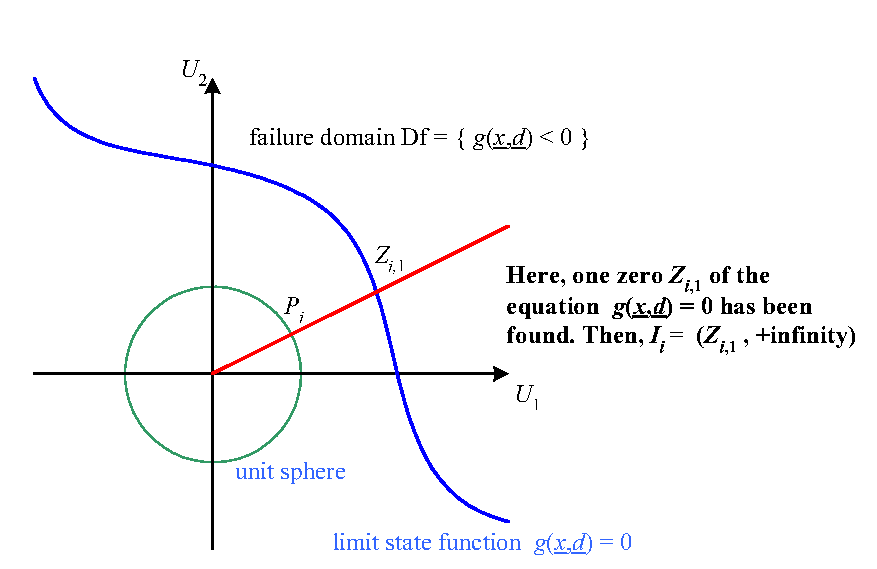
\includegraphics[scale=1]{Figures/Sdir.pdf}
  \end{center}

  The Central Limit Theorem enables the difference between the estimated value and the sought value to be controlled by means of a confidence interval (if N is sufficiently large, typically $N$ > a few dozens even if there is now way to say for sure if the asymptotic behaviour is reached). For a probability $\alpha$ strictly between 0 and 1 chosen by the user, one can, for example, be sure with a confidence $\alpha$, that the true value of $P_f$ is between $\widehat{P}_{f,\inf}$ and $\widehat{P}_{f,\sup}$ calculated analytically from simple formulae. To illustrate, for $\alpha = 0.95$:
  \begin{align*}
    \widehat{P}_{f,\inf} = \widehat{P}_{f,DS} - 1.96 \frac{\sigma_q}{\sqrt{N}},\ \widehat{P}_{f,\sup} = \widehat{P}_{f,DS} + 1.96 \frac{\sigma_q}{\sqrt{N}}
  \end{align*}
  \begin{align*}
    \textrm{that is to say}\ \Prob{ \widehat{P}_{f,\inf} \leq P_f \leq \widehat{P}_{f,\sup}} = 0.95
  \end{align*}
  where $\sigma_q$ denotes the empirical standard deviation of the sample $\left\{ q_1,\ldots,q_N \right\}$.

  In practice in OpenTURNS, the Directional Sampling simulation requires the choice of:
  \begin{itemize}
  \item[$\bullet$] a Root Strategy :
    \begin{itemize}
    \item  RiskyAndFast : for each direction, we check whether there is a sign changement of the standard limit state function between the maximum distant point (at distance {\itshape MaximumDistance} from the center of the standard space) and the center of the standard space. \\
      In case of sign changement, we research one root in the segment [origin, maximum distant point] with the selected non linear solver.\\
      As soon as founded, the segment [root, infinity point] is considered within the failure space.

    \item MediumSafe : for each direction, we go along the direction by step of length {\itshape stepSize} from the origin to the maximum distant point (at distance {\itshape MaximumDistance} from the center of the standard space) and we check whether there is a sign changement on each segment so formed.\\
      At the first sign changement, we research one root in the concerned segment with the selected non linear solver. Then, the segment [root, maximum distant point] is considered within the failure space. \\
      If {\itshape stepSize} is small enough, this strategy garantees us to find the root which is the nearest from the origin.

    \item SafeAndSlow : for each direction, we go along the direction by step of length {\itshape stepSize} from the origin to the maximum distant point(at distance {\itshape MaximumDistance} from the center of the standard space) and we check whether there is a sign changement on each segment so formed.\\
      We go until the maximum distant point.  Then, for all the segments where we detected the presence of a root, we research the root with the selected non linear solver. We evaluate the contribution to the failure probability of each segment. \\
      If {\itshape stepSize} is small enough, this strategy garantees us to find all the roots in the direction and the contribution of this direction to the failure probability is precisely evaluated.
    \end{itemize}

  \item[$\bullet$] a Non Linear Solver :
    \begin{itemize}
    \item Bisection : bisection algorithm,
    \item Secant : based on the evaluation of a segment between the two last iterated points,
    \item Brent : mix of Bisection, Secant and inverse quadratic interpolation.
    \end{itemize}
  \item[$\bullet$] and a Sampling Strategy :
    \begin{itemize}
    \item RandomDirection : we generate some points on the sphere unity according to the uniform distribution and we consider both opposite directions so formed.
    \item OrthogonalDirection : this strategy is parameterized by $k\in \{1,\dots,n\}$, where $n$ is the dimension of the input random vector $\vect{X}$. We generate one direct orthonormalized basis $(e_1, \dots, e_n)$ uniformly distributed in the set of direct orthonormal bases. We consider all the normalized linear combinations of $k$ vectors chosen within the $n$ vectors of the basis, where the coefficients of the linear combinations are in $\{+1, -1\}$. This generates $C_n^k 2^k$ new vectors $v_i$. We sample according to all the directions defined by the vectors $v_i$.\\
      If $k=1$, we consider all the axes of the standard space.
    \end{itemize}
  \end{itemize}
}
{
}

\Methodology{
  This method is used in step C and enables the probability of exceeding the threshold of an output variable (we refer to the probability of exceeding the threshold (critical region) because the inequality $g(\vect{X},\vect{d}) \le 0$ by convention defines a reliability/critical region, and is in the general case the rewritten inequality of type $Z \geq \textrm{threshold}$ where $Z$ is a random variable function of $\vect{X}$ and $\vect{d}$).

  This amounts to calculating the cumulative distribution function of the output variable at a point and thus propagating the uncertainty defined in step B using the model defined in step A.\\

  Input data:
  \begin{itemize}
  \item $\vect{X}$: random vector modelling the unknown variables defined in step A and for which the joint probability density function has been defined in step B,
  \item $\vect{d}$: vector of deterministic calculation parameters,
  \item $g(\vect{X},\vect{d})<0$: probabilistic criterion specified in step A,
  \end{itemize}

  Parameters:
  \begin{itemize}
  \item $N$: number of simulations,
  \item $\alpha$: confidence level required for the confidence interval,
  \item Root Strategy,
  \item Non-linear Solver,
  \item Sampling Strategy.
  \end{itemize}

  Outputs:
  \begin{itemize}
  \item $\widehat{P}_{f,DS}$: estimation of the probability of exceeding the threshold,
  \item $\textrm{Var}({\widehat{P}_f})$: estimation of the variance of the probability estimator,
  \item $\widehat{P}_{f,\sup}-\widehat{P}_{f,\inf}$: length of the confidence interval.
  \end{itemize}
}
{
  Readers interested in the problem of estimating the probability of exceeding a threshold are also referred to \otref{docref_C311_Form}{FORM}, \otref{docref_C311_Sorm}{SORM}, \otref{docref_C322_LHS}{LHS}, \otref{docref_C322_TI}{Importance Sampling} and \otref{docref_C321_MonteCarloStd}{Crude Monte-Carlo sampling}.

  The following provide an interesting bibliographical starting point to further study of this method:
  \begin{itemize}
  \item Robert C.P., Casella G. (2004). Monte-Carlo Statistical Methods, Springer, ISBN 0-387-21239-6, 2nd ed.
  \item Rubinstein R.Y. (1981). Simulation and The Monte-Carlo methods, John Wiley \& Sons
  \item Bjerager, P. (1988). "Probability integration by Directional Simulation". Journal of Engineering Mechanics, vol. 114, no. 8
  \end{itemize}
}
